\section{Auswertung}
Die Temperaturen $T_{1}$ und $T_{2}$ wurden in dem Experiment in Celsius gemessen und können anschließend in Kelvin umgerechnet werden, was die Berechnung
der gesuchten Größen ermöglicht. Die Temperaturverläufe seien in dem folgedenen Diagramm \ref{fig:plot1} skizziert.
\begin{figure}[h]
  \centering
  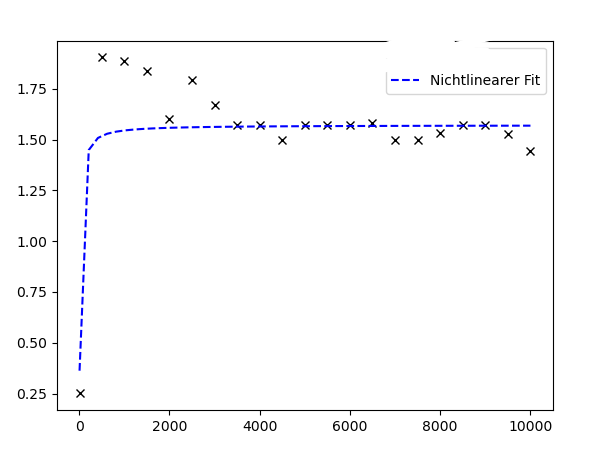
\includegraphics[width=\textwidth]{build/plot1.pdf}
  \caption{Messdaten der Temperaturen}
  \label{fig:plot1}
\end{figure}
\begin{flushleft}
Dabei wurde die Abzisse als Zeit $t$ in Sekunden gewählt. Nun lässt sich eine Ausgleichsfunktion durch
die einzelnen Messwerte legen, dafür wurde hier ein Polynomansatz zweiten Grades gewählt. Also
\end{flushleft}
\begin{equation}
T(t) = \symup{A} t^{2} + \symup{B} t + \symup{C}
\end{equation}
Die Parameter, inklusive Fehler, lassen sich beispielsweise mit einem curvefit in python berechnen.
Für die erste Ausgleichsfunktion $T_{1}$($t$) entstehen folgende Parameter
\begin{align}
A_{1} &= (-3.22 \pm 0.042)\cdot 10^{-6} \, \si[per-mode=symbol]{\kelvin\per\second\squared}\\
B_{1} &= (20 \pm 0.091) 10^{-3} \,\si[per-mode=symbol]{\kelvin\per\second}\\
C_{1} &= (294.97 \pm 0.042) \,\si{\kelvin}
\end{align}
Analog erhält man für die Ausgleichsfunktion $T_{2}$($t$) die Parameter
\begin{align}
A_{2} &= (9.55 \pm 2.67)\cdot 10^{-7} \, \si[per-mode=symbol]{\kelvin\per\second\squared}\\
B_{2} &= (-11.20 \pm 0.58) 10^{-3} \,\si[per-mode=symbol]{\kelvin\per\second}\\
C_{2} &= (295.87 \pm 0.26) \,\si{\kelvin}
\end{align}
Wenn man diese Funktionen nun in das Diagramm \ref{fig:plot1} einfügt, erkennt man,
dass die Parameter plausibel sind.
\begin{figure}[h]
  \centering
  \includegraphics[width=\textwidth]{build/plot2.pdf}
  \caption{Messdaten der Temperaturen und Ausgleichsfunktionen}
  \label{fig:plot2}
\end{figure}